\section{OS Security}

\begin{description}
    \item[OS Security Goals] secrecy, integrity, availability
    \item[Trust Model] set of SW and data which the system depends on for correct enforcement of security goals
    \item[Threat Model] set of operations available to compromise system
\end{description}

\subsection{Access control}
Whether to allow requests from \textbf{subjects} to perform \textbf{operations} on \textbf{objects}.

\begin{description}
    \item[protection system] defines security requirements of OS. Consists of protection state and protection state operations
        \begin{description}
            \item[protection state] operations a subject can perform on obj.
            \item[protection state operations] enable modification of state
        \end{description}
\end{description}

An access matrix defines which operations a subject can perform on an obj. (subject as row, object as column)
Store by column: ACL (\textbf{A}ccess \textbf{C}ontrol \textbf{L}ist) stored with objects.
Store by row: Capability of a subject
\begin{center}
    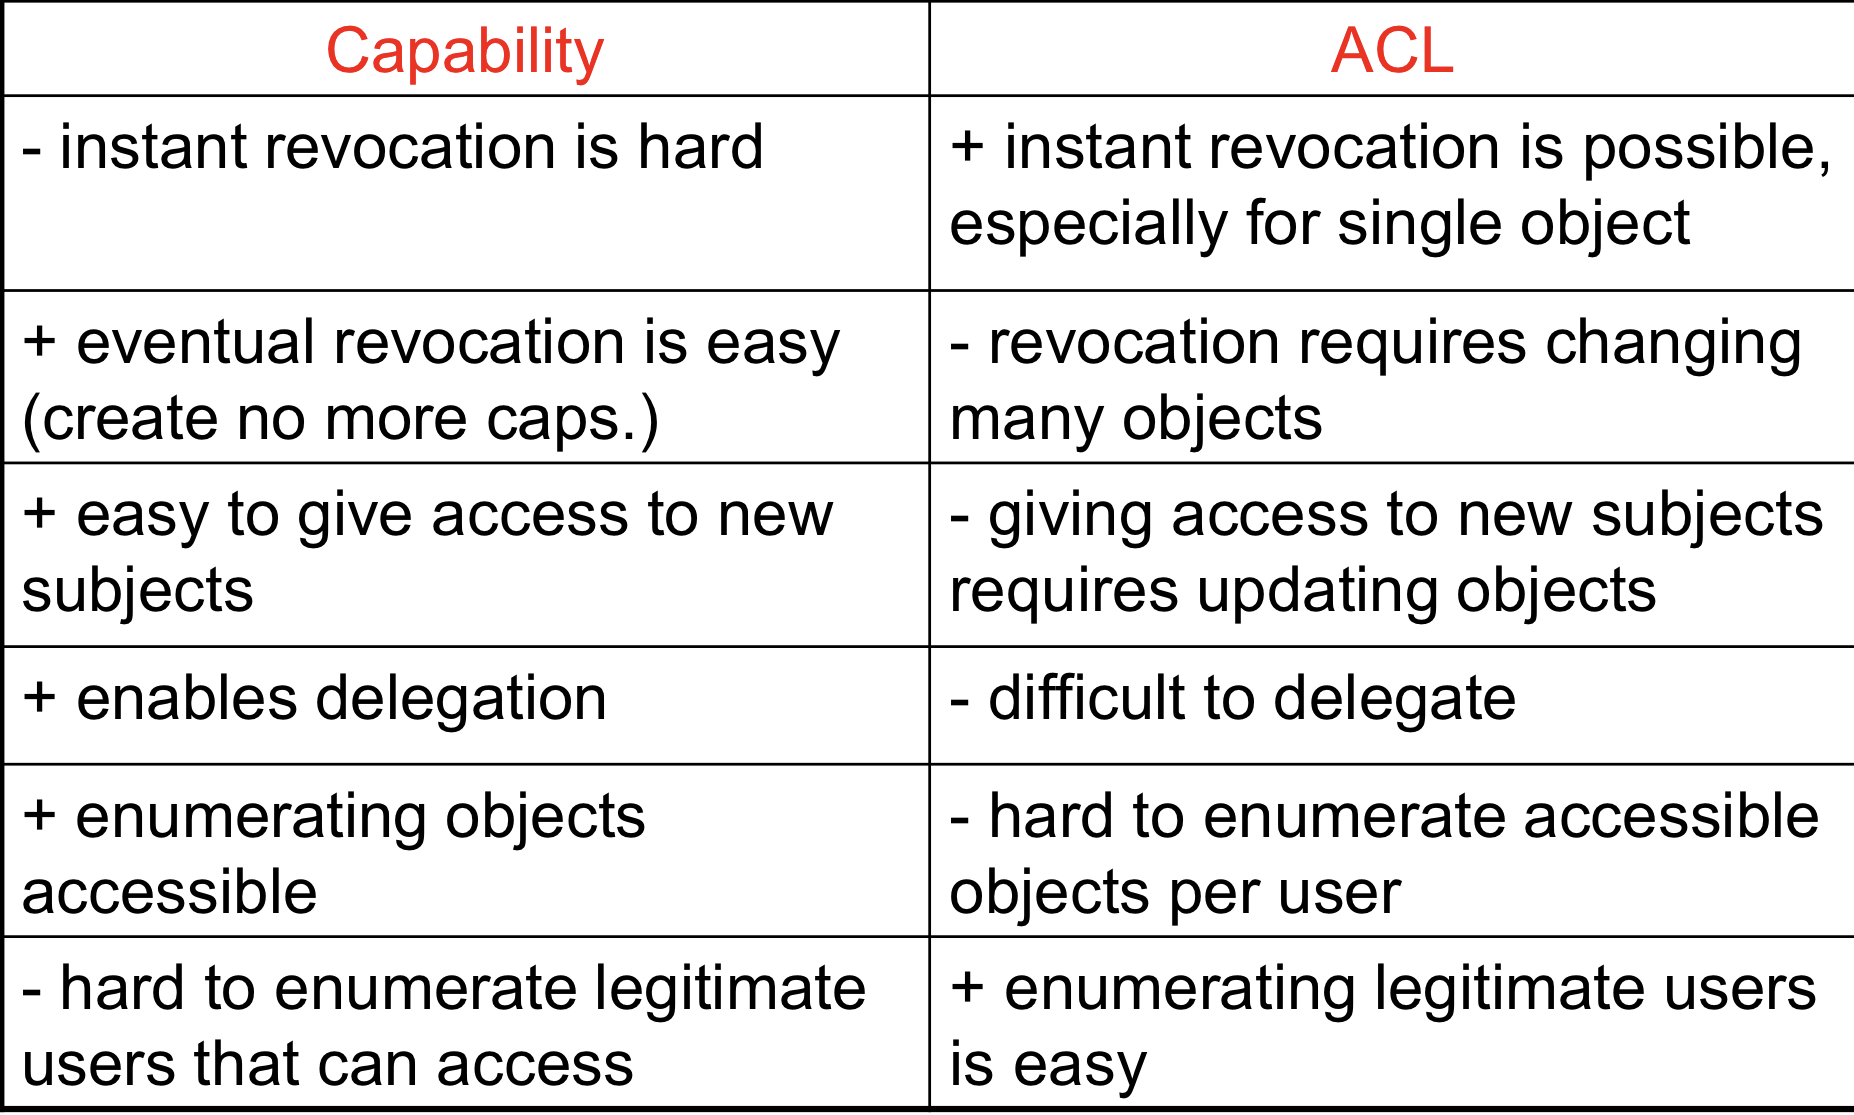
\includegraphics[width=0.65\linewidth]{images/os_sec_capabilities-vs-ACLs.png}
\end{center}

\subsubsection{DAC}
\textbf{D}iscretionary \textbf{A}ccess \textbf{C}ontrol.
Is called discretionary, because subject can pass on his permissions directly/indirectly to other subjects.
\begin{itemize}
    \item allow untrusted processes/users to modify protection state
    \item only works if all processes are harmless and users make no mistakes
\end{itemize}
\subsubsection{MAC}
\textbf{M}andatory \textbf{A}ccess \textbf{Control}

\begin{itemize}
    \item only modifiable by admin
    \item subjects and obj are labels, state represents allowed operations
    \item transition state is legal way to relabel subjects and objs
\end{itemize}

\begin{center}
    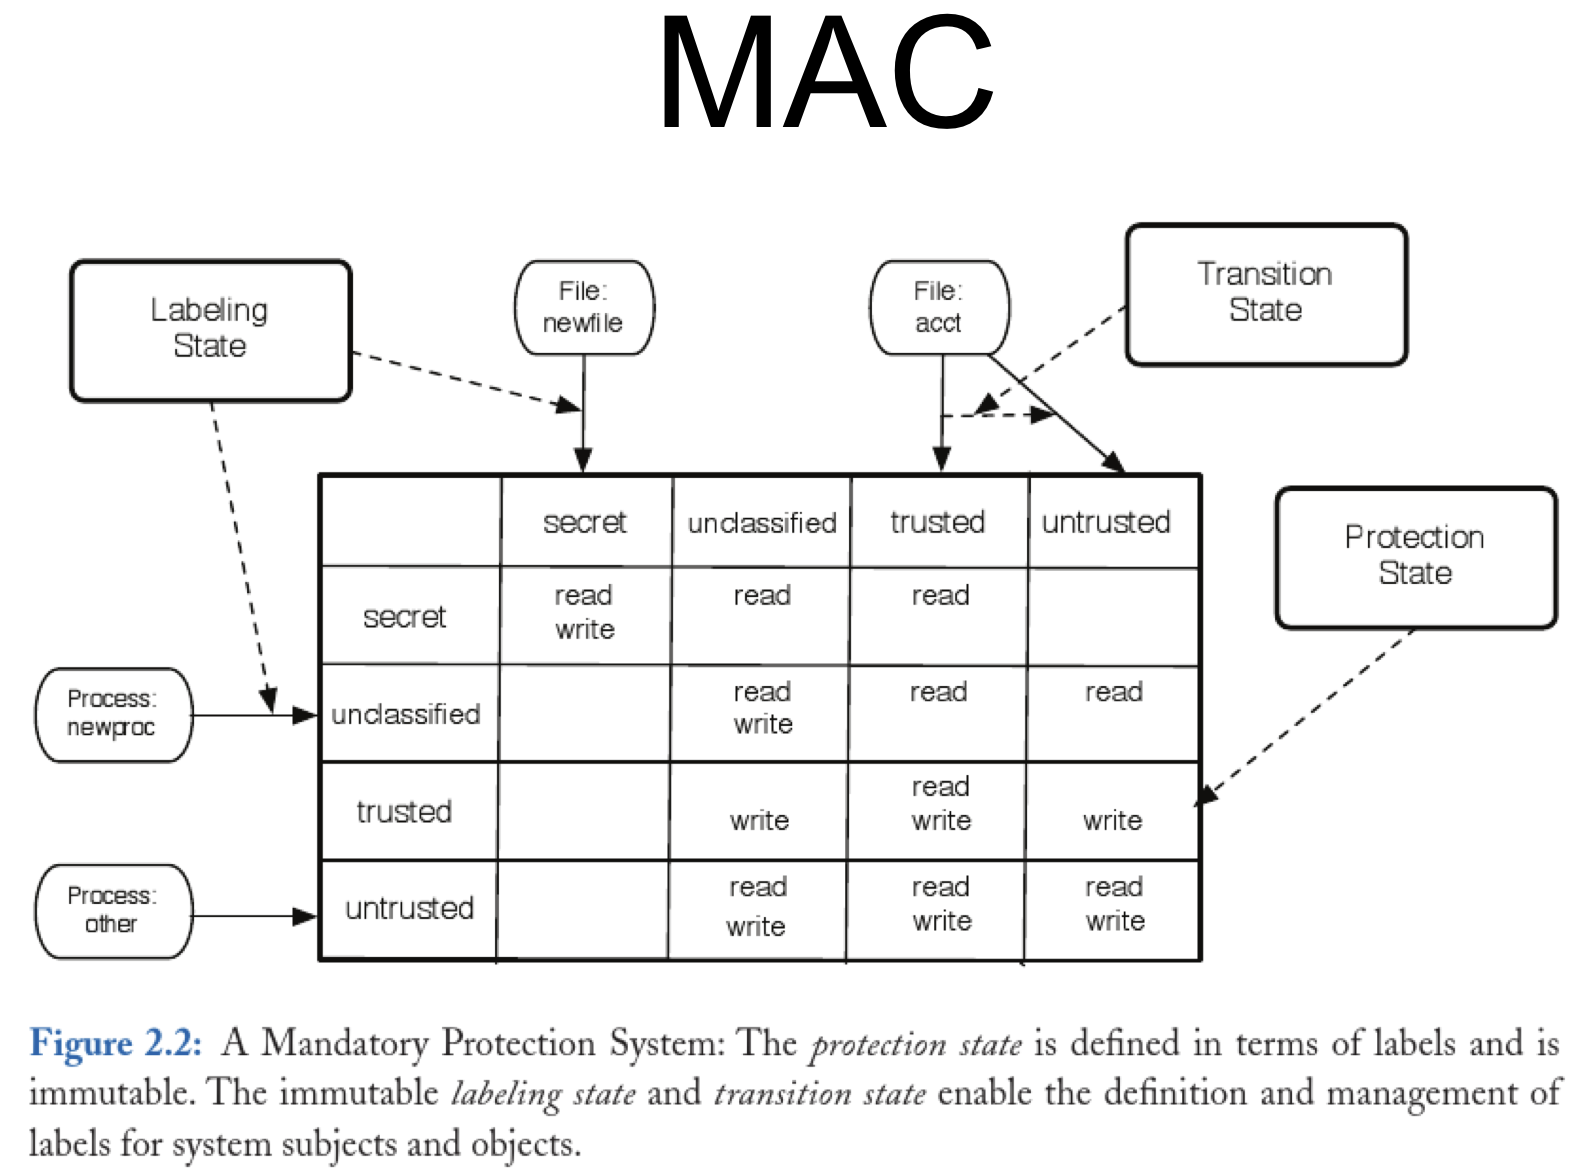
\includegraphics[width=0.9\linewidth]{images/os_sec_MAC.png}
\end{center}

\subsubsection{Reference Monitor}
\begin{description}
    \item[input] request of security sensitive operation
    \item[output] binary answer
    \item[authorization module] converts request into query for policy store
\end{description}

\textbf{Secure OS} iff system uses reference monitor which satisfies:
\begin{enumerate}
    \item complete mediation
    \item tamperproof
    \item verifiable
\end{enumerate}

Does not protect against TOCTTOU attacks.

\subsubsection{Covert Channels}
Capability to transfer information between processes that are not supposed to be allowed to communicate by the security policy.

There are \textbf{storage} and \textbf{timing} channels.

Prevent it by:
\begin{itemize}
    \item memoryless program
    \item isolate program
    \item transitivity (if program A is confined and calls program B, then B must also be confined)
    \item masking (caller determines all inputs to all channels)
    \item enforcement (enforce that input into covert channel conforms with caller's [security] specification)
\end{itemize}

\subsection{Unix Access Control}
\subsubsection{Chmod}
Only the owner  of a file (or \texttt{root}) can change file permissions. Even if a user has write access via group permissions he is not able to change it.
\subsubsection{Setuid}
When an executable file's \texttt{setuid} permission is set, users may execute that
program with a level of access that matches the user who owns the file.

The kernel ignores \texttt{setuid} on scripts for security reasons.
\subsubsection{Directory Permissions}
\begin{description}
  \item[read bit (\texttt{r})(\texttt{4})] allows to list the files within the directory
  \item[write bit (\texttt{w})(\texttt{2})] allows to create, rename, or delete files
    within the directory, and modify the directory's attributes
  \item[execute bit (\texttt{x})(\texttt{1})] allows  to enter the directory, and access files and directories inside (without execute permission we can \textbf{not} list, write or create files in the directory)
  \item[sticky bit (\texttt{T}, or \texttt{t} if the execute bit is set for
    \texttt{others})] states that files and directories within that directory
    may only be deleted or renamed by their owner (or root)
  \item[setuid] no effects
  \item[setgid] causes any file created in a directory to inherit the
    directory's group
\end{description}

\subsubsection{\texttt{sudo}, \texttt{su}}

\texttt{sudo}:
\begin{itemize}
  \item used to gain root access using the user's own password.
  \item users with sudo access defined in \texttt{/etc/sudoers} or part of \texttt{sudo} group.
\end{itemize}
\texttt{su}:
\begin{itemize}
  \item used to switch between users using the target user's password
\end{itemize}
\texttt{sudo} allows more fine-grained configuration and thereby more selective
privilege escalation. $\Rightarrow$ prefer \texttt{sudo} over \texttt{su}.

\subsection{Linux Security Model}
Process in user space has access rights based on user ID (UID).

UID 0 is reserved for \texttt{root}.
\begin{description}
    \item[kernel process] can access everything
    \item[root process] can order kernel process to access everything
\end{description}

Kernel verifies permissions before system call! Compares UID and GID (Group ID) of subject and object.

\subsubsection{Password change}
\begin{itemize}
  \item \texttt{/bin/passwd} has suid bit set and thus runs as root.
  \item This is needed to change the passwords in \texttt{/etc/passwd}.
  \item \texttt{/bin/passwd} can access \textbf{any} system ressource.
  \item $\Rightarrow$ must trust \texttt{/bin/passwd}
\end{itemize}
Many programs can run as root and thus can modify the
shadow password file!


\subsection{SELinux}
No default superuser exists, because SELinuxs default is to deny access. Everything must be specifically granted.

\subsubsection{RBAC: Role based access control}
\begin{itemize}
  \item rules specify roles user can use
  \item rules specify when and where a user can transition into another role
\end{itemize}

\subsubsection{MLS:  multi level security}
\begin{itemize}
  \item handling of classified data where \textit{no read up} or \textit{write down} is allowed
  \item enforce by file system labeling
\end{itemize}

\subsubsection{Modes}
SELinux has the following modes:

\begin{description}
  \item[Disabled:] loaded, but not running. Only DAC is enforced
  \item[Permissive:]  Policy is not enforced, but would-be denials are logged
  \item[Enforcing:] Policy is enforced, access is denied based on rules
\end{description}
\subsubsection{Type enforcement}

In SELinux every subject/object has a \textbf{security context} which consists of three labels:\vspace{-1.5mm}
\begin{description}
    \item[user label] on a subject: user privileges, on an object: objects owner
    \item[role label]  on a subject: subject's role, on an object: no meaning (always defaults to \texttt{object\char`_r})
    \item[domain label] set of subjects and objects which are allowed to interact with each other
\end{description}
This is called \textbf{type enforcement}! SELinux can make two types of decisions:\vspace{-1.5mm}
\begin{description}
    \item[access decision] Is subject allowed to do something within it's domain?
    \item[transition decision] Is subject allowed to do somthing in another domain (transition into this domain)?
\end{description}
Hard part is not to grant access to files, but allowing \textbf{safe domain transitions}.

\subsubsection{Allow rule}
four elements:
\begin{description}
  \item[Source type:] Domain type of a process attempting access
  \item[Target type:] Type of an object being accessed by the process
  \item[Object class:] Class of object that the specified access is permitted
  \item[Permission:] Kind of access that the source type is allowed
\end{description}

Example rule for passwd (access to shadow file missing):\\
\texttt{allow user\char`_t passwd\char`_exec\char`_t: file $\{$ getattr execute $\}$; \\ allow passwd\char`_t passwd\char`_exec\char`_t: file entrypoint; \\ allow user\char`_t passwd\char`_t: process transition;}

\subsubsection{System call}
\begin{center}
  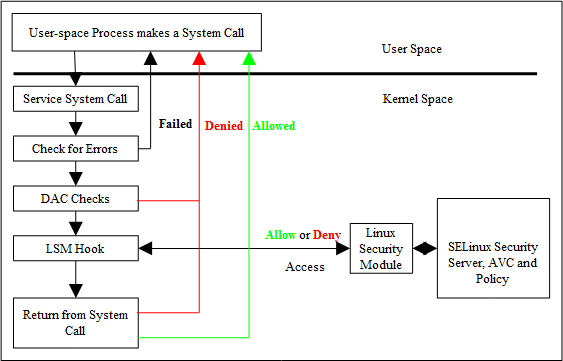
\includegraphics[width= 0.7\columnwidth]{os_sec_system-call.png}
\end{center}

\subsection{Other OSs}
\subsubsection{Qubes}
Security by compartmentalization. 1 qube equals 1 VM.

\subsubsection{Microkernels}
Idea is to minimize TCB. Follows least priviledge principle and removes many parts from kernel space.
\begin{center}
    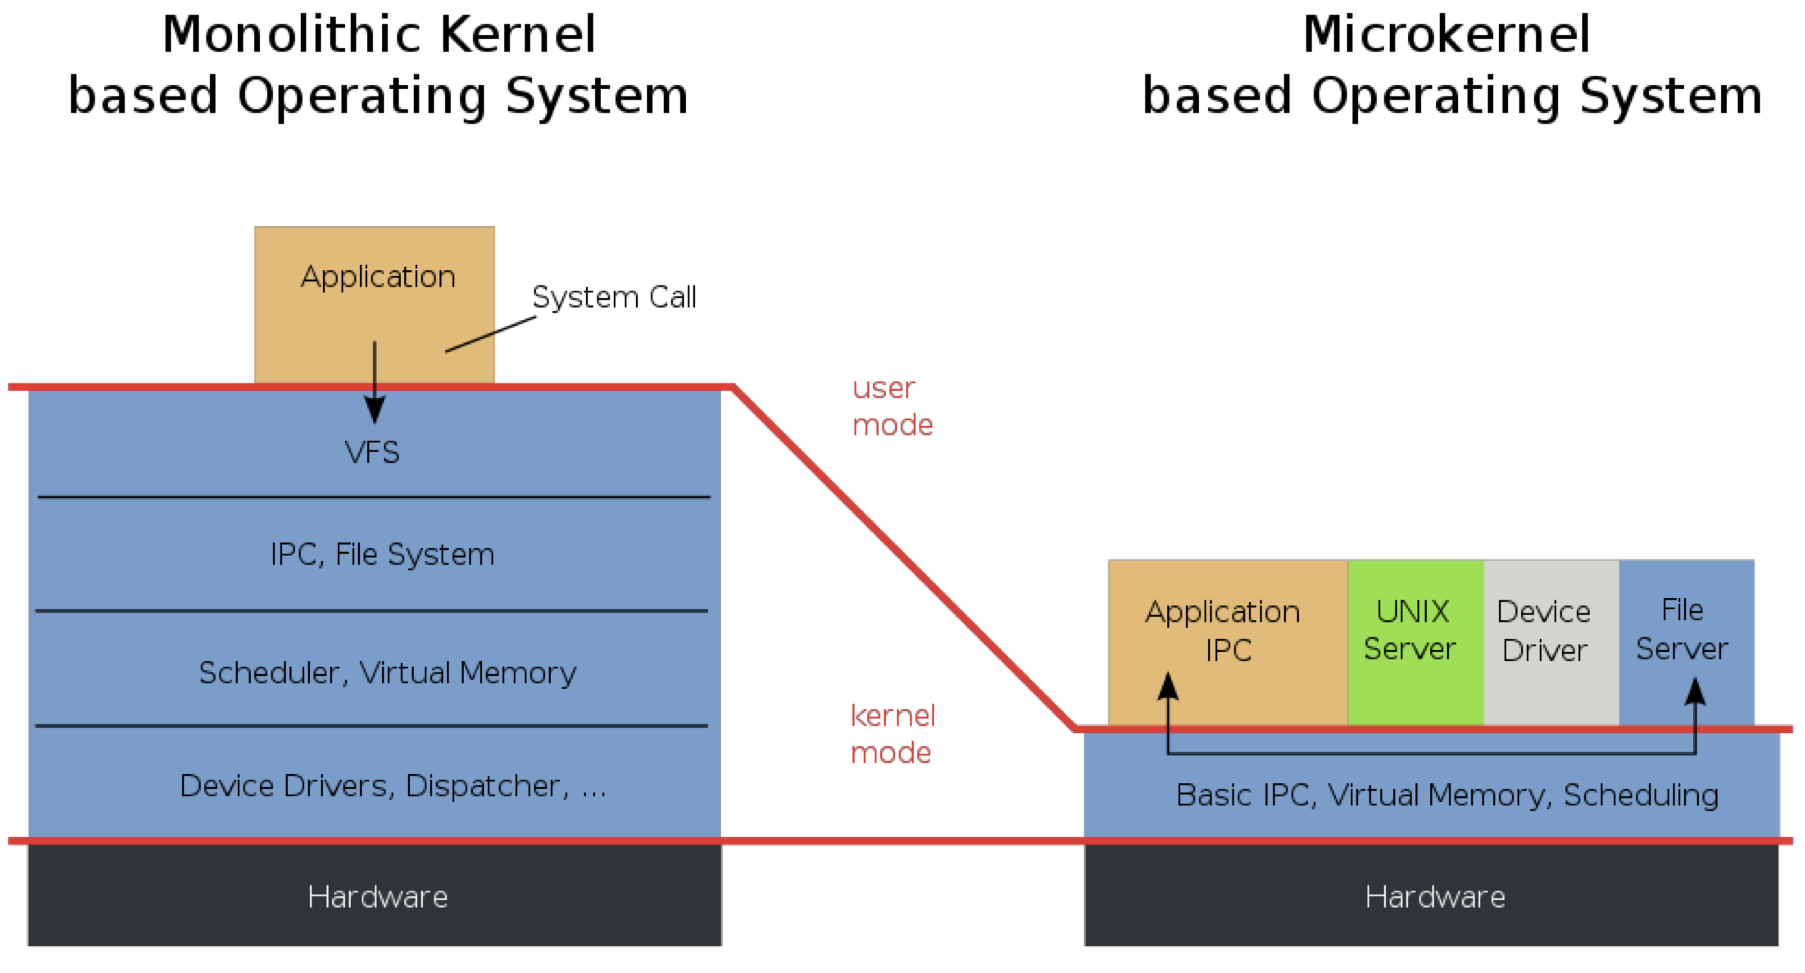
\includegraphics[width=0.8\linewidth]{images/os_sec_MicrokernelVSMonolithic.png}
\end{center}

\textbf{sel4} is a microkernel which focuses on efficency and high assurance. Uses formal verification of code to guarantee correctness w.r.t. specification.
